%% Pattern Recognition Letters submission draft
%% Class: elsarticle (final, 5p, two-column, times)
%% Compile: tectonic main.tex  (or via the pdf skill wrapper)
%% Status: camera-ready (rev F). Numbers = frozen canonical ledger (post-supersession);
%%         expkit outputs (E9-E14) integrated; no pending markers remain.
%% Rev E (2nd external review round): (1) GriTS-Top ordering claim corrected --
%%         it sides with TEDS-S (0.7908 vs 0.7605), not with F1; (2) LORE K=100
%%         cap reframed as a constraint, not the proven cause of the plateau;
%%         (3) Sec. 3.2 states per-system ground truth (TATR = separate
%%         PubTables-1M sample); (4) OSF registration claims REMOVED (never
%%         registered -- protocol is pre-specified and released via the repo);
%%         (5) Contribution 2 pins the 406-TP reference to snap-disabled matching.
%% Rev F: all \subsection headers removed -- the letter runs as continuous
%%         prose inside numbered sections; the four subsection cross-refs
%%         (Table 2 / Table 4 captions, Limitations) now point to the parent
%%         sections. No text, numbers, or findings changed.
%% Rev G: methodology overview figure added (fig:method, TikZ, full-width);
%%         referenced from the first sentence of the Audit design section.
\documentclass[final,5p,times,twocolumn]{elsarticle}

\usepackage{amsmath,amssymb}
\usepackage{graphicx}
\usepackage{tikz}
\usetikzlibrary{arrows.meta,positioning,fit,calc}
\usepackage{booktabs}
\usepackage{tabularx}
\usepackage{adjustbox}
\usepackage{xcolor}
\usepackage[colorlinks=true,linkcolor=blue,citecolor=blue,urlcolor=blue,bookmarks=true]{hyperref}

%% elsarticle forces \ttdefault=cmtt (cls line 87), which has no TU font
%% definition under Tectonic/XeTeX: \texttt silently renders as roman and
%% paragraphs containing it are broken with phantom metrics. Latin Modern
%% Typewriter resolves cleanly under TU.
\renewcommand{\ttdefault}{lmtt}

%% The `times' class option loads txfonts, but only OT1 metrics exist in the
%% bundle: every TU/txr text shape is undefined, so all text silently falls
%% back to Latin Modern (upright), while some font *requests* (e.g. the
%% italic style leaked by elsarticle's italic subsection headings) are broken
%% with mismatched phantom metrics, producing badness-10000 lines. Aliasing
%% the txr family onto the resolved lmr shapes makes breaking metrics match
%% rendered glyphs without changing the document's appearance.
\DeclareFontFamily{TU}{txr}{}
\DeclareFontShape{TU}{txr}{m}{n}{<->sub*lmr/m/n}{}
\DeclareFontShape{TU}{txr}{m}{it}{<->sub*lmr/m/n}{}
\DeclareFontShape{TU}{txr}{m}{sl}{<->sub*lmr/m/n}{}
\DeclareFontShape{TU}{txr}{m}{sc}{<->sub*lmr/m/n}{}
\DeclareFontShape{TU}{txr}{m}{ui}{<->sub*lmr/m/n}{}
\DeclareFontShape{TU}{txr}{b}{n}{<->sub*lmr/bx/n}{}
\DeclareFontShape{TU}{txr}{b}{it}{<->sub*lmr/bx/n}{}
\DeclareFontShape{TU}{txr}{b}{sl}{<->sub*lmr/bx/n}{}
\DeclareFontShape{TU}{txr}{bx}{n}{<->sub*lmr/bx/n}{}
\DeclareFontShape{TU}{txr}{bx}{it}{<->sub*lmr/bx/n}{}
\DeclareFontShape{TU}{txr}{bx}{sl}{<->sub*lmr/bx/n}{}

\newcommand{\ie}{i.e.}
\newcommand{\eg}{e.g.}

\widowpenalty=10000
\clubpenalty=10000
\emergencystretch=3.5em
\raggedbottom
\hyphenation{Table-Former Pub-TabNet Table-Trans-for-mer set-pack-ing post-pro-cess-ing re-pro-du-ci-bi-li-ty equ-iva-lence}

\biboptions{numbers,sort&compress}

\journal{Pattern Recognition Letters}

\begin{document}
\begin{frontmatter}

\title{Post-processing and evaluation artifacts dominate measured losses in table
       structure recognition: a cross-paradigm audit}

\author[a]{Abhinav Shukla\corref{cor1}\fnref{fn1}}
\ead{student2.ai@csvtu.ac.in}
\cortext[cor1]{Corresponding author.}
\fntext[fn1]{ORCID: 0009-0001-8471-8604}
\author[a]{Nachiket Tapas\fnref{fn2}}
\fntext[fn2]{ORCID: 0000-0002-7860-8572}
\affiliation[a]{organization={Department of Computer Science \& Engineering,
                Chhattisgarh Swami Vivekanand Technical University},
                city={Bhilai}, country={India}}

\begin{abstract}
Table structure recognition (TSR) pipelines couple a learned model with
hand-designed or optimized post-processing, and benchmark numbers silently
conflate model error with downstream losses and evaluation-pipeline artifacts. We audit four public TSR paradigms---a
split-and-merge heuristic pipeline (SPLERGE), a transformer with snap-to-text
matching (TableFormer, docling), a detection
transformer with conflict suppression (TATR), and a logical-location
regression network (LORE)---under trace-level instrumentation on 100 PubTabNet
tables (5{,}646 ground-truth cells; PubTables-1M for the detection
arm); a pre-specified 1{,}000-table replication
follows. It isolates four artifacts. (1)~SPLERGE's merge heuristic
destroys 27.1\% (OCR) to 34.4\% (oracle) of valid cells; an exact
set-packing ILP restores the raw grid's true-positive count (1{,}836
vs.\ 1{,}833; 71 wins, 0 losses) while improving
F1. (2)~Under the same objective, unnormalized greedy collapses
to 27.5\% of exact recall while footprint-normalized greedy matches the ILP:
objective design, not solver exactness, binds. (3)~LORE's headline recall
deficit is a threshold-policy artifact: lowering the confidence threshold
$\tau$ from 0.35 to 0.20 lifts recall from 31.2\% to 90.5\% at 99.2\%
precision without model changes, and recall plateaus below
$\tau{\approx}0.1$. (4)~TableFormer's PDF text layer is synthesized from ground-truth boxes;
snapping to it inflates the oracle-token count by 406 over
snap-disabled matching (circularity), whereas exact maximum-weight independent set selection on OCR
tokens matches the raw count (TOST $\pm 2$~TP,
$p=5.5\times 10^{-117}$). Finally, TEDS-S rewards over-pruning: the destructive heuristic
outscores exact selection on 57 of 100 tables (+0.059 mean TEDS-S) while
destroying 500 valid cells. We release traces, the frozen ledger, and the replication protocol.
\end{abstract}

\begin{keyword}
table structure recognition \sep evaluation methodology \sep post-processing
\sep set packing \sep maximum weight independent set \sep reproducibility
\end{keyword}

\end{frontmatter}

%% ------------------------------------------------------------------
\section{Introduction}\label{sec:intro}

Table structure recognition (TSR) systems convert the image of a table into a
machine-readable cell topology, and modern pipelines almost universally pair a
learned model with a non-trivial post-processing stage: split-and-merge
heuristics~\cite{zhong2020,tensmeyer2019}, coordinate snapping inside a
matching post-processor~\cite{nassar2022tableformer,auer2024docling},
score-thresholded conflict resolution~\cite{smock2022pubtables1m}, and
confidence-thresholded candidate emission~\cite{xing2023lore}. Benchmark
protocol then measures the composed system against ground truth with a chosen
metric~\cite{zhong2020,smock2023grits}. Each of these three layers---model,
post-processor, evaluation---can introduce errors, yet published evaluations
report only their convolution. When a reported number moves, the community
attributes the change to the model or to the method---without decomposing the
pipeline, neither attribution is justified.

This paper asks a narrow but consequential question: \emph{how much of the
measured behaviour of published TSR pipelines is attributable to the learned
model at all, and how much is manufactured downstream?} We answer it with a
cross-paradigm audit of four publicly released systems spanning the main
paradigm families---grid-based split-and-merge (SPLERGE),
transformer-with-matching (TableFormer), detection-transformer-with-NMS
(TableTransformer, TATR), and logical-location regression (LORE)---instrumented
at the trace level. Every intermediate representation is
frozen: raw grids, heuristic merge operations, candidate graphs, solver
outputs, matched true positives. We then replace each heuristic component with
an exact combinatorial formulation under \emph{identical inputs and an
identical objective}, and measure what changes. Where a difference appears, we
test whether it is significant with a pre-fixed statistical protocol; where a
difference vanishes, we test whether it is \emph{equivalent} using TOST rather
than claiming it from a failed significance test.

The audit surfaces four artifacts, each of which inverts a plausible reading
of the published numbers. First, the SPLERGE merge heuristic is not a benign
clean-up: it destroys between 27.1\% and 34.4\% of the valid cells produced by
its own split stage, and an exact set-packing formulation recovers the raw
count with zero losses against the heuristic (71 wins, 29 ties, 0 losses).
Second, the exact solver is not what matters in that comparison: an
unnormalized greedy heuristic under the same objective collapses to a quarter
of exact recall, while a footprint-normalized greedy matches the ILP
exactly---the binding constraint is objective design, not computational
exactness. Third, LORE's apparent recall deficit is a policy artifact: the
published threshold discards candidates the detector itself ranks highly, and
one threshold change recovers most of the deficit at essentially unchanged
precision. Fourth, and most damaging for
evaluation practice, the TableFormer evaluation corpus used by the docling
toolchain synthesizes its PDF text layer \emph{from ground-truth cell
boxes}~\cite{auer2024docling}; its matching post-processor snaps predictions
onto that layer, so a portion of the reported accuracy is circular. On top of
the four artifacts we document a metric pathology: tree-edit-distance
structure scoring (TEDS-S) rewards the destructive heuristic over the exact
one on 57 of our 100 tables.

\paragraph{Scope and positioning.} This is a measurement-validity study, not a
state-of-the-art claim. Our audit corpus is deliberately fixed at 100
PubTabNet tables (5{,}646 ground-truth cells) so that every intervention is
traceable cell by cell, and all N=100 analyses are labelled exploratory. The
confirmatory instrument---a 1{,}000-table, stratified, pre-specified
replication with pinned seeds, pinned dependencies and pre-committed decision
rules---is released before execution (Section~\ref{sec:prereg}). Absolute scores on our audit subset are therefore
not comparable to published leaderboard numbers; every claim concerns
\emph{within-pipeline} contrasts between conditions that share data, models,
and metrics.

\paragraph{Contributions.}
\begin{enumerate}
\item A trace-level, cross-paradigm audit methodology for TSR pipelines, with a
      canonical cell-matching procedure and a frozen results ledger that makes
      every reported number re-derivable from committed artifacts.
\item Four isolated artifacts with effect sizes and significance/equivalence
      tests: destructive merge heuristics (27--34\% cell destruction, raw TP
      count restored by set packing); objective-vs-solver dissociation (unnormalized
      greedy collapse to 27.5\%, normalized greedy = ILP); threshold-policy
      recall deficit (31.2\%$\to$90.5\% recall from one threshold); and
      evaluation circularity through ground-truth-derived text layers
      (+406~TP inflation over snap-disabled matching, removed by exact
      selection on OCR tokens).
\item A multi-metric divergence analysis showing that TEDS-S rewards
      over-pruning systematically rather than anecdotally (heuristic wins on
      57/100 tables, Wilcoxon $p = 2.5\times 10^{-3}$; 7\% of tables lose
      over half their cells yet score $\geq 0.80$, including one where the
      heuristic retains 3.9\% of cells yet scores 0.9265), and that
      F1 orders the same systems in the opposite direction while
      GriTS-Top repeats the TEDS-S ordering.
\item A pre-specified 1{,}000-table replication with pre-committed
      hypotheses, TOST margins, power analysis (minimum detectable effect
      0.75~TP/table at $\alpha{=}0.01$, 80\% power) and a pinned sampling
      fallback, to be executed before journal acceptance.
\end{enumerate}

%% ------------------------------------------------------------------
\section{Related work}\label{sec:related}

\paragraph{TSR paradigms.} Grid-based methods predict a table grid and then
merge elementary cells into spans; SPLERGE~\cite{tensmeyer2019} formalizes
this as a split network followed by a hand-designed merging stage, and the
PubTabNet corpus with the GraphTSR model and the TEDS metric was introduced in
the same line of work~\cite{zhong2020}. Transformer-based structure
recognizers such as TableFormer~\cite{nassar2022tableformer} predict cell
boxes and HTML structure and rely on a matching post-processor that snaps
sloppy coordinates onto known text
tokens~\cite{nassar2022tableformer,auer2024docling}. Detection-transformer
approaches such as the TableTransformer (TATR)~\cite{smock2022pubtables1m}
emit row/column boxes resolved by score-maximizing conflict suppression.
Logical-location regression methods such as
LORE~\cite{xing2023lore} predict logical positions of cells directly and emit
candidates under a confidence threshold. End-to-end and hybrid systems
(\eg\ TSRFormer~\cite{song2022tsrformer}) pursue the same compositionality
with different mechanisms.

\paragraph{Metrics.} TEDS and TEDS-S score tree-edit distance between HTML
predictions and ground truth~\cite{zhong2020}; GriTS scores table similarity
directly in matrix form, with topology (GriTS-Top) and content (GriTS-Con)
variants~\cite{smock2023grits}. Cell-level true positives at a fixed IoU
threshold remain the de-facto primitive of most published tables, yet these
metrics are not interchangeable even at the sign level: the
same pair of systems is ordered oppositely by F1 and by TEDS-S or GriTS-Top,
making single-metric leaderboard claims fragile.

\paragraph{Evaluation-validity studies.} Prior work in table recognition has
largely focused on model improvement; systematic studies of how
post-processing and evaluation mechanics shape reported results are rare and
typically confined to a single system. To our knowledge this is the first
cross-paradigm audit that (i) replaces each heuristic with an exact
formulation under a frozen objective, (ii) separates exploratory from
pre-specified confirmatory analyses, and (iii) publishes a frozen ledger with
supersession tracking so that number drift (\eg\ between a figure and a
table) is detectable rather than silent.

%% ------------------------------------------------------------------
\section{Audit design}\label{sec:design}

\begin{figure*}[t]
\centering
\resizebox{\textwidth}{!}{%
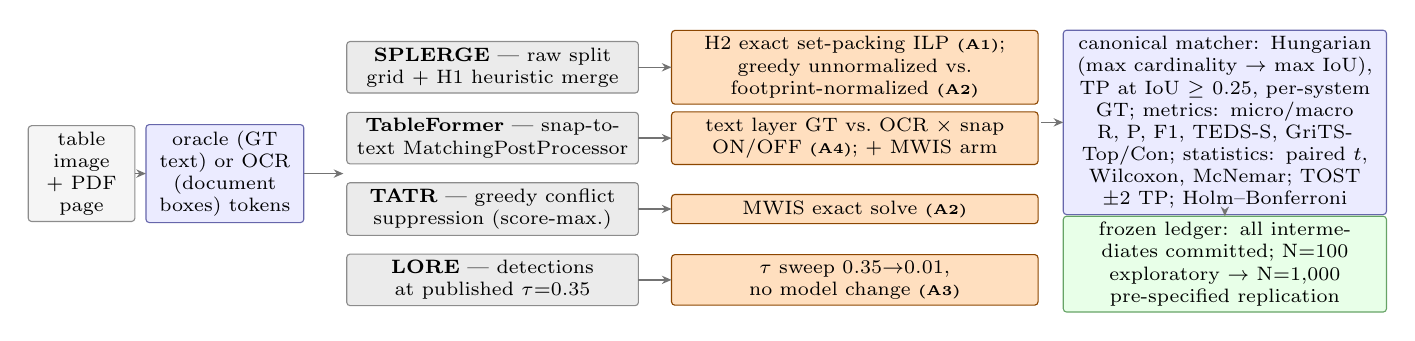
\begin{tikzpicture}[
  font=\scriptsize,
  cell/.style={draw=black!45, line width=0.4pt, rounded corners=1.2pt, align=center, inner sep=2.2pt, outer sep=0pt},
  pub/.style={cell, fill=black!8, text width=3.55cm},
  aud/.style={cell, fill=orange!25, draw=orange!55!black, text width=4.5cm},
  meas/.style={cell, fill=blue!8, draw=blue!45!black!60},
  led/.style={cell, fill=green!9, draw=green!40!black!60, text width=3.95cm},
  ar/.style={-{Stealth[length=3.5pt,width=3pt]}, black!55, line width=0.5pt}
]
% ---- left: input and token conditions --------------------------------
\node[cell, fill=black!4, text width=1.2cm] (input) at (0.73,-1.8) {table image + PDF page};
\node[cell, fill=blue!8, draw=blue!45!black!60, text width=1.85cm] (toks) at (2.55,-1.8) {oracle (GT text) or OCR (document boxes) tokens};
% ---- middle: four paradigm lanes -------------------------------------
\node[pub] (p1) at (5.95,-0.45) {\textbf{SPLERGE} --- raw split grid + H1 heuristic merge};
\node[aud] (a1) at (10.55,-0.45) {H2 exact set-packing ILP~{\tiny\bfseries(A1)}; greedy unnormalized vs.\ footprint-normalized~{\tiny\bfseries(A2)}};
\node[pub] (p2) at (5.95,-1.35) {\textbf{TableFormer} --- snap-to-text MatchingPostProcessor};
\node[aud] (a2) at (10.55,-1.35) {text layer GT vs.\ OCR $\times$ snap ON/OFF~{\tiny\bfseries(A4)}; + MWIS arm};
\node[pub] (p3) at (5.95,-2.25) {\textbf{TATR} --- greedy conflict suppression (score-max.)};
\node[aud] (a3) at (10.55,-2.25) {MWIS exact solve~{\tiny\bfseries(A2)}};
\node[pub] (p4) at (5.95,-3.15) {\textbf{LORE} --- detections at published $\tau{=}0.35$};
\node[aud] (a4) at (10.55,-3.15) {$\tau$ sweep $0.35{\to}0.01$, no model change~{\tiny\bfseries(A3)}};
\draw[ar] (p1.east) -- (a1.west); \draw[ar] (p2.east) -- (a2.west);
\draw[ar] (p3.east) -- (a3.west); \draw[ar] (p4.east) -- (a4.west);
% ---- right: measurement stack ----------------------------------------
\node[meas, text width=3.95cm] (box1) at (15.25,-1.15)
 {canonical matcher: Hungarian (max cardinality $\rightarrow$ max IoU), TP at IoU $\geq 0.25$, per-system GT; metrics: micro/macro R, P, F1, TEDS-S, GriTS-Top/Con; statistics: paired $t$, Wilcoxon, McNemar; TOST $\pm2$~TP; Holm--Bonferroni};
\node[led] (box2) at (15.25,-2.95)
 {frozen ledger: all intermediates committed; N=100 exploratory $\rightarrow$ N=1{,}000 pre-specified replication};
\draw[ar] (box1.south) -- (box2.north);
% ---- flow arrows ------------------------------------------------------
\draw[ar] (input.east) -- (toks.west);
\node[draw=none, inner sep=1pt, fit=(p1)(a1)(p4)(a4)] (lanes) {};
\draw[ar] (toks.east) -- (lanes.west |- toks);
\draw[ar] (lanes.east |- box1.west) -- (box1.west);
\end{tikzpicture}}%
\caption{Audit methodology. Gray: published configurations (one public
pipeline per paradigm), run under oracle and OCR tokens. Orange: audited
arms---A1 exact set packing vs.\ the merge heuristic; A2 solver dissociation
under a frozen objective; A3 LORE's confidence-threshold sweep (no model
change); A4 TableFormer's text layer (GT vs.\ OCR) $\times$ snap ON/OFF, plus
an MWIS arm. Blue: canonical Hungarian matching (TP at IoU $\geq 0.25$,
per-system GT) feeding the metric suite, paired tests, and TOST equivalence.
Green: all intermediates committed to the frozen ledger ahead of the
pre-specified N=1{,}000 replication.}
\label{fig:method}
\end{figure*}

We audit four systems spanning the paradigm space (Fig.~\ref{fig:method}): the SPLERGE
split-and-merge pipeline~\cite{tensmeyer2019} executed through its five-stage
reference merge module (v2; per-stage attribution in
Table~\ref{tab:trace}); the
TableFormer model as packaged in docling-models v2.1.0 with its matching
post-processor~\cite{nassar2022tableformer,auer2024docling}; the
TableTransformer structure recognition model v1.1 (TATR)~\cite{smock2022pubtables1m}
with its standard conflict-resolution settings; and
LORE-TSR~\cite{xing2023lore} with its published detection threshold
$\tau{=}0.35$. Exact function names for every stage are in the released code
and frozen ledger.

All model evaluations employ publicly released checkpoints without local
fine-tuning or retraining. SPLERGE uses the pretrained split-stage model
\texttt{split\_model\_\allowbreak pubtabnet.pth} of the reference
implementation~\cite{tensmeyer2019}, with the five-stage merge module
re-executed from its released code. TableFormer uses IBM's
\texttt{docling-models} v2.1.0 release~\cite{auer2024docling} with checkpoint
\texttt{tableformer/\allowbreak model.safetensors}. TATR uses the HuggingFace release
\texttt{microsoft/\allowbreak table-\allowbreak transformer-\allowbreak
structure-\allowbreak recognition-\allowbreak v1.1-all}, revision
\texttt{54eb6a5}~\cite{smock2022pubtables1m}. LORE uses the official
LORE-TSR release~\cite{xing2023lore} with its PubTabNet-trained checkpoint
\texttt{ckpt\_ptn/\allowbreak model\_best.pth}.
Checkpoint provenance affects absolute scores, not artifact directions:
every claim remains a \emph{within-pipeline contrast} under fixed inputs. Model loading and inference
use pinned dependencies (Python~3.12, \texttt{torch}~2.5.1, \texttt{scipy}~1.15.1
with HiGHS branch-and-cut, \texttt{apted}~1.0.3, \texttt{lxml}~5.3.0,
\texttt{pymupdf}~1.25.1); all solver inputs and outputs are committed to the
frozen ledger.

The audit corpus is 100 tables sampled from PubTabNet~\cite{zhong2020},
containing 5{,}646 ground-truth cells; the TATR arm uses a 100-table
PubTables-1M test sample~\cite{smock2022pubtables1m}. Each pipeline is run
under two token conditions: \emph{oracle} tokens (ground-truth text with
predicted geometry, isolating the post-processor) and \emph{realistic} OCR
tokens (document-extracted token boxes, the deployable configuration). All
conditions of a given system are scored against that system's own ground
truth with one canonical matcher: predicted and ground-truth cells are paired
by maximum cardinality and then maximum total IoU (Hungarian algorithm), and
a pair counts as a true positive at IoU $\geq 0.25$. The three PubTabNet arms
thus share the 5{,}646-cell ground-truth set, whereas the TATR arm is scored
against its separate PubTables-1M sample; every reported contrast remains
within-pipeline. We report micro-recall (total TPs
over the 5{,}646-cell denominator), macro-recall (mean per-table recall),
precision, F1, TEDS-S~\cite{zhong2020}, and GriTS-Top~\cite{smock2023grits}.
GriTS-Con is reported only under oracle tokens: under OCR tokens the audit's
token extractor emits placeholder strings, reducing GriTS-Con to a
character-count artifact---we document rather than publish this failure mode. The official LORE matcher (first-come bipartite
assignment) and the canonical matcher were verified to produce identical
true-positive counts on every table ($\Delta = 0$~TP), with no ambiguous
(multiple-optimal) assignments ($0/100$ tables).

The analysis protocol was fixed before the multi-metric suite was executed;
the N=100 results below are therefore protocol-frozen but
\emph{exploratory}---the confirmatory, pre-specified analyses are the
1{,}000-table ones (Section~\ref{sec:prereg}). Paired comparisons use the
paired $t$-test and the Wilcoxon signed-rank test; discordant-count
comparisons use exact McNemar; family-wise error is controlled by
Holm--Bonferroni step-down at $\alpha{=}0.05$~\cite{holm1979}. Where our claim
is the \emph{absence} of an effect, we use two-one-sided-tests (TOST)
equivalence testing~\cite{lakens2017} with a pre-specified margin of
$\pm 2$~TP per table, chosen \emph{before} the TableFormer comparisons as
3.54\% of the mean table size (56.46 cells)---the ambiguity of at most a
single $1\times 2$ sub-cell boundary---and not recalibrated afterwards.
Solver-side claims are validated by construction: the exact set-packing
solutions are verified integral (HiGHS branch-and-cut, zero fractional
solutions), and a nine-configuration sensitivity sweep over the objective's
regularization constants (each varied across one order of magnitude) leaves
the selected cell set's TP count unchanged at 1{,}836 in all nine
configurations; regularization terms are $\sim$1\% of the dominant
token-coverage weights.
Mean solve times are 60.3~ms per table (ILP) and 4.2~ms per table (MWIS);
exactness is computationally affordable at audit scale.

%% ------------------------------------------------------------------
\section{Findings}\label{sec:findings}

Table~\ref{tab:metrics} is the audit's centerpiece: every condition is scored
with the full metric suite under identical matching. Three facts are
immediate. First, the SPLERGE heuristic is destructive in both token
conditions: relative to the raw split grid (1{,}833 TPs), heuristic merging
retains only 1{,}203 TPs under oracle tokens ($-34.4\%$) and 1{,}336 under
OCR tokens ($-27.1\%$). Second, replacing the heuristic with an exact
set-packing ILP over the same candidate graph restores the raw count:
1{,}836 TPs in both token conditions (count-level recovery: the ILP's
selected cell sets need not coincide with the raw grid's), with a paired
advantage of
$+5.00$~cells/table over the heuristic ($t(99)=6.66$,
$p=1.5\times 10^{-9}$; Wilcoxon $p=2.2\times 10^{-13}$; 71 wins, 29 ties,
0 losses). Third, the exact solution wins the pooled operational metric: it
improves F1 substantially (28.7\% vs.\ 26.3\% under OCR; 28.8\% vs.\ 24.1\%
under oracle tokens), while precision moves by at most $\pm 0.40$~pp (27.49\%
vs.\ 27.89\% under OCR, 27.68\% vs.\ 27.38\% under oracle) and GriTS-Top stays
within $+0.003$ of the raw grid (Table~\ref{tab:metrics}), so the repair is
not an artifact of recall-chasing alone.

The merge-stage trace completes the mechanism: instrumenting the heuristic
operation by operation quantifies \emph{how many merges it performs and how
many are wrong}. Each removed separator is scored against ground-truth cell
edges: a removal is \emph{incorrect} when ground-truth cells carry an edge at
the removed position across more than half of the table width, \ie\ the merge
fused two cells that ground truth keeps separate. On the exact side, every
ILP-selected multi-tile merge is classified by whether all of its elementary
tiles fall inside a single ground-truth cell. Table~\ref{tab:trace} shows the
result: of 318 merge operations applied across the five stages, 41 (12.9\%)
are incorrect, and the damage concentrates in \texttt{row\_merging} (80.0\%
of its 10 operations) and the first redundant-separator pass (27 incorrect of
209); the ILP, by contrast, selects 69 multi-tile merges of which 72.5\%
(50/69) fall entirely inside one ground-truth cell.

\begin{table}[t]
\centering
\footnotesize
\caption{Merge-stage attribution for the SPLERGE heuristic (100 tables, OCR
token condition). Ops = merge operations applied at the stage (separator
removals, header merges); incorrect = ops that fused cells across a
ground-truth edge present over $>$50\% of the table width.}
\label{tab:trace}
\begin{tabular*}{\columnwidth}{@{\extracolsep{\fill}} l r r r}
\toprule
Stage & Ops & Incorrect & Inc.\ (\%) \\
\midrule
col\_merging      & 1   & 0  & 0.0  \\
row\_merging      & 10  & 8  & 80.0 \\
remove\_seps 0.2  & 209 & 27 & 12.9 \\
remove\_seps 0.4  & 27  & 6  & 22.2 \\
merge\_header\_v2 & 71  & 0  & 0.0  \\
\midrule
All stages        & 318 & 41 & 12.9 \\
\bottomrule
\end{tabular*}
\end{table}

Destruction concentrates where it matters: stratifying tables by the fraction
of spanning cells, the heuristic's destruction rate rises from 26.7\% (low)
through 33.6\% (medium) to 36.6\% (high), while exact selection recovers
100.0\%, 100.0\% and 99.6\% of raw TPs in the same strata; the correlation
between spanning complexity and destruction is weak but significant (Pearson
$r=0.297$, $p=0.0027$; Spearman $\rho=0.307$, $p=0.0019$). In other words,
the more a table needs spans, the more the heuristic loses.

\begin{table*}[t]
\centering
\footnotesize
\caption{Multi-metric audit results on 100 PubTabNet tables (5{,}646
ground-truth cells). H1/H2 denote heuristic vs.\ exact set-packing selection;
token condition in parentheses (GT = oracle tokens, OCR = realistic tokens).
GriTS-Con is reported only under oracle tokens (see
Section~\ref{sec:design}). Greedy = unnormalized greedy selection under the
ILP objective (Section~\ref{sec:findings}). TP counts are corpus totals; Micro/Macro R are corpus-level and mean
per-table recall; precision and F1 are per-table means.}
\label{tab:metrics}
\begin{tabular*}{\textwidth}{@{\extracolsep{\fill}} l r r r r r c c c}
\toprule
Condition & TP & Micro & Macro & Prec & F1 & TEDS-S & GriTS-Top & GriTS-Con \\
 & & R (\%) & R (\%) & (\%) & (\%) & & & \\
\midrule
Raw split grid         & 1{,}833 & 32.47 & 33.81 & 27.16 & 28.42 & 0.6680 & 0.7575 & -- \\
H1 heuristic (GT)      & 1{,}203 & 21.31 & 23.06 & 27.38 & 24.11 & 0.6888 & 0.7633 & 0.6042 \\
H2 exact, ILP (GT)     & 1{,}836 & 32.52 & 33.96 & 27.68 & 28.82 & 0.6733 & 0.7594 & 0.6212 \\
H1 heuristic (OCR)     & 1{,}336 & 23.66 & 26.02 & 27.89 & 26.29 & 0.7318 & 0.7908 & -- \\
H2 exact, ILP (OCR)    & 1{,}836 & 32.52 & 33.96 & 27.49 & 28.72 & 0.6725 & 0.7605 & -- \\
Greedy, unnorm.\ (OCR) & 504\textsuperscript{$\dagger$} & 8.93 & 10.68 & 13.15 & 10.74 & 0.4230 & 0.5629 & -- \\
\bottomrule
\end{tabular*}
\par\smallskip
\noindent\footnotesize \textsuperscript{$\dagger$}Canonical seed-42
unnormalized greedy; the superseded 566 arose from unjittered tie-breaking.
Under footprint normalization ($w_i / |\text{tiles}_i|$), greedy selection
recovers 1{,}836~TP, matching the exact ILP.
\end{table*}

The natural objection to Artifact 1 is that exactness itself is the
contribution. It is not. Holding the candidate graph and the objective
(token-coverage weights with fixed regularization) fixed, three solvers
disagree dramatically. Unnormalized greedy---select candidates in descending
total weight subject to tile disjointness---collapses to 504 TPs, 27.5\% of
exact recall, and correspondingly wrecks every metric (TEDS-S 0.4230,
GriTS-Top 0.5629). The collapse is robust to tie-breaking: the superseded
unjittered ordering yields 566~TP (Table~\ref{tab:metrics}, footnote
$\dagger$) and the canonical jittered seed-42 ordering 504~TP, both under a
third of exact recall. A footprint-normalized greedy
(sorting by weight per covered tile) recovers to 1{,}836 TPs and matches the
ILP's selections almost everywhere. The mechanism is over-commitment: large
multi-tile merges carry the largest total weights, so unnormalized greedy
locks them in early and forecloses sets of elementary tiles whose aggregate
weight is higher---a knapsack-style failure that normalization removes.

Where conflicts are rare, exactness and greed agree, and the audit quantifies
how rare ``rare'' is. On the TATR arm (PubTables-1M sample; 1{,}867 row/column
candidates across 100 tables; conflict criterion: same-axis overlap ratio
$\geq 0.25$ at detection score $\geq 0.5$; TP matching at IoU 0.25), the
conflict graph decomposes into isolated singletons for 97.98\% of candidate
vertices and 10 isolated $K_2$ pairs, in which greedy suppression is provably
optimal; the residual components are short alternating paths of length
$\geq 3$, and no component with a clique of size $\geq 3$ occurs anywhere in
the corpus. Greedy score-maximizing suppression and exact maximum-weight
independent set differ on a single table
(\texttt{PMC6127715\_table\_0}), worth $+1$~TP in total. Paired significance
testing confirms this honest null: exact two-sided McNemar $p = 1.0000$
(1 win, 0 losses, 99 ties), Wilcoxon signed-rank (normal approximation, one nonzero pair) $p = 0.3173$ ($W = 0.0$),
paired $t(99) = 1.000$, $p = 0.3197$, and a bootstrap 95\% CI on the paired
mean difference of $[+0.0000, +0.0300]$~TP/table. The audit's conclusion is
therefore symmetric and
solver-agnostic: \emph{objective design dominates wherever conflict structure
is rich (SPLERGE), and is immaterial wherever it is trivial (TATR)}; exact
solvers matter because they remove the need for per-pipeline normalization
tricks.

LORE-TSR ships with detection confidence $\tau{=}0.35$. Sweeping $\tau$ over
the audit corpus with no model change (Table~\ref{tab:lore}) shows that the
headline recall deficit is a policy artifact: at $\tau{=}0.35$ the detector
emits 1{,}778 candidates (31.2\% recall, 99.0\% precision); at $\tau{=}0.20$
it emits 5{,}153 candidates with 90.5\% recall at \emph{higher} precision
(99.2\%), F1 94.7\%. Per-table paired tests confirm that the recovery
carries no precision penalty: cell TP rises by $+33.50$ cells/table (100
wins, 0 losses, 0 ties; paired $t(99) = 16.790$, $p = 1.002\times 10^{-30}$;
Wilcoxon $p = 3.861\times 10^{-18}$; bootstrap 95\% CI $[+29.66, +37.50]$),
the mean paired precision difference is negligible ($+0.02$~pp, $t(99) =
0.063$, $p = 0.9501$), and mean paired F1 rises by $+52.93$~pp ($t(99) =
25.904$, $p = 6.821\times 10^{-46}$). The
recovery is free because the detector already ranks those candidates highly;
the threshold simply discards them.

Two genuine ceilings appear, and both are upstream of any post-processing.
Below $\tau{\approx}0.10$, recall plateaus at 91.75\% while false positives
explode $269\times$ (17 $\to$ 4{,}576 from $\tau{=}0.35$ to $\tau{=}0.01$),
collapsing precision to 53.1\%; true positives stay fixed at 5{,}180 for all
$\tau \leq 0.10$, so no threshold policy recovers the residual 466 cells.
CenterNet's fixed query budget $K{=}100$---which caps the per-table candidate
pool, bounding achievable recall on tables with more than 100 cells---is one
structural constraint consistent with the plateau; attributing the plateau to
the cap would require re-running detection with an enlarged query budget,
which we did not attempt. Post-processing cannot repair either ceiling.
The correct reading
of Table~\ref{tab:lore} is that a third of LORE's ``model error'' on this
corpus is a configurable emission policy---and that tuning it moves LORE's
operating point across an F1 range wider than many published model
improvements.

\begin{table*}[t]
\centering
\footnotesize
\caption{LORE-TSR confidence-threshold sweep on the 100-table audit corpus
(5{,}646 ground-truth cells); no model changes. The published default is
$\tau{=}0.35$ (bold). Below $\tau{\approx}0.10$ recall plateaus
and precision collapses.}
\label{tab:lore}
\begin{tabular*}{\textwidth}{@{\extracolsep{\fill}} r r r r r r r r}
\toprule
$\tau$ & Predictions & TP & FP & FN & Precision (\%) & Recall (\%) & F1 (\%) \\
\midrule
0.50           & 1{,}371 & 1{,}357 & 14    & 4{,}289 & 98.98 & 24.03 & 38.68 \\
0.40           & 1{,}385 & 1{,}368 & 17    & 4{,}278 & 98.77 & 24.23 & 38.91 \\
\textbf{0.35}  & \textbf{1{,}778} & \textbf{1{,}761} & \textbf{17} & \textbf{3{,}885} & \textbf{99.04} & \textbf{31.19} & \textbf{47.44} \\
0.30           & 2{,}965 & 2{,}944 & 21    & 2{,}702 & 99.29 & 52.14 & 68.38 \\
0.25           & 4{,}276 & 4{,}250 & 26    & 1{,}396 & 99.39 & 75.27 & 85.67 \\
\textbf{0.20}  & \textbf{5{,}153} & \textbf{5{,}111} & \textbf{42} & \textbf{535} & \textbf{99.18} & \textbf{90.52} & \textbf{94.66} \\
0.15           & 5{,}246 & 5{,}176 & 70    & 470 & 98.67 & 91.68 & 95.04 \\
0.10           & 5{,}313 & 5{,}180 & 133   & 466 & 97.50 & 91.75 & 94.53 \\
0.05           & 5{,}983 & 5{,}180 & 803   & 466 & 86.58 & 91.75 & 89.09 \\
0.01           & 9{,}756 & 5{,}180 & 4{,}576 & 466 & 53.10 & 91.75 & 67.26 \\
\bottomrule
\end{tabular*}
\end{table*}

The docling-models evaluation path (v2.1.0) for
TableFormer~\cite{nassar2022tableformer,auer2024docling} constructs its PDF
text layer \emph{from ground-truth cell boxes}; the \texttt{MatchingPostProcessor}
then snaps predicted cell coordinates onto those tokens. Any TP counted after
snapping has been scored against coordinates derived from ground truth---a
circular measurement channel. We quantify this with a $2\times 2$ factorial
(Table~\ref{tab:tableformer}): token source (ground-truth layer vs.\ OCR) crossed
with snapping (on/off), plus an exact-selection arm. Snapping inflates the
oracle-token count by 406 TPs (5{,}488 vs.\ 5{,}082 snap-off), and depresses the
OCR-token count by 1{,}019 (3{,}902 vs.\ 4{,}921): the same mechanism that
manufactures accuracy when the text layer is ground truth destroys real
detections when it is not.

\begin{table}[t]
\centering
\footnotesize
\caption{TableFormer factorial audit (docling-models v2.1.0; corpus TP totals).
$\dagger$: the snapped-to-ground-truth count is circular by construction
(Section~\ref{sec:findings}). MWIS = maximum-weight independent set over the
candidate graph, exact solve.}
\label{tab:tableformer}
\begin{tabular*}{\columnwidth}{@{\extracolsep{\fill}} l r r}
\toprule
Configuration & TP & $\Delta$ vs.\ raw \\
\midrule
Raw (published; GT layer)   & 5{,}204 & -- \\
GT layer, snap ON$^\dagger$ & 5{,}488 & +406 vs.\ snap-OFF \\
GT layer, snap OFF          & 5{,}082 & $-122$ \\
OCR, snap ON                & 3{,}902 & $-1{,}019$ vs.\ snap-OFF \\
OCR, snap OFF               & 4{,}921 & $-283$ \\
OCR, snap OFF + MWIS        & 5{,}202 & $+281$ vs.\ 4{,}921 \\
\bottomrule
\end{tabular*}
\end{table}

The exact arm closes the loop. Selecting cells by maximum-weight independent
set over the OCR-token candidate graph (no snapping, no ground-truth
contact) rescues $+281$ TPs over the snap-disabled OCR baseline
($t=4.28$, $p=4.4\times 10^{-5}$; 42 wins, 55 ties, 3 losses) and is
statistically \emph{equivalent} to the raw published count (5{,}202 vs.\
5{,}204; TOST, pre-specified margin $\pm2$~TP, $p=5.5\times 10^{-117}$).
The methodological lesson generalizes beyond this one toolchain: when an
evaluation artifact contains ground-truth information, every component that
touches it inherits leakage; exact selection over raw predictions removes the
channel.

\paragraph{Honest disclosure of procedure.} The conflict criterion used by the
snap-disabled pipeline was selected in a \emph{diagnostic} phase that did read
ground truth: source tracing revealed a 190-TP loss attributable to the
original criterion, and 28 tolerance settings were evaluated during that
diagnosis. To show that the GT-informed choice cannot manufacture the
confirmatory result, two-one-sided-tests (TOST; per-table paired, $df{=}99$)
equivalence checking against
the pre-specified margin $\Delta_0 = \pm 2.0$~TP/table was run across all 28
coordinate-tolerance configurations ($dx \in \{0, 2, 5, 8\}$~pt, $dy \in
\{0, 1, 3, 5, 10, 15, 20\}$~pt): all 28 pass ($28/28$, $100.0\%$; maximum
$p_{\mathrm{TOST}} = 9.33 \times 10^{-12}$; maximum observed mean
$|\Delta| = 0.710$~TP/table). We state the two-phase structure explicitly
rather than claim the criterion was chosen blind.

The final audit finding is that the field's default structure metric orders
the systems in the opposite direction from every operational metric. On the
100-table corpus under OCR tokens, the destructive heuristic outscores exact
selection on TEDS-S (0.7318 vs.\ 0.6725) and GriTS-Top (0.7908 vs.\ 0.7605)
while destroying 500 valid cells and losing on precision, F1, and
GriTS-Con under oracle tokens (0.6042 vs.\ 0.6212, $p=1.0\times 10^{-6}$).
The mechanism is structural: the split stage over-segments, so the heuristic's
aggressive row pruning moves the predicted tree's size toward the
ground-truth tree, and tree edit distance rewards the pruning itself.

Because isolated cases do not establish how often this occurs, we paired the
two selection rules on every table and scored the per-table TEDS-S
difference under a destruction/score grid fixed before the sweep. The divergence is
corpus-wide rather than anecdotal: the heuristic outscores exact selection
on 57 of 100 tables (9 ties, 34 losses; Wilcoxon signed-rank
$p = 2.5\times 10^{-3}$; paired $t(99) = 2.92$, $p = 4.4\times 10^{-3}$), a
mean paired advantage of $+0.0593$ TEDS-S purchased with 500 destroyed true
positives (5.0 per table). Table~\ref{tab:prevalence} applies the
pre-declared grid: among the 38 tables where the heuristic destroys at
least 30\% of the cells that exact selection recovers, 11 (11\% of the
corpus) still score $\geq 0.80$ TEDS-S under the heuristic; the
corresponding counts at $\geq 50\%$ and $\geq 70\%$ destruction are 7 of 29
and 1 of 15. Fig.~\ref{fig:teds-scatter} shows that the advantage is not
coupled to the scale of destruction: if TEDS-S penalized cell loss,
per-table advantages would fall below zero as destroyed cells accumulate;
instead the association is weak and statistically indistinguishable from
zero (Pearson $r = -0.095$, $p = 0.35$; Spearman $\rho = -0.138$,
$p = 0.18$), and tables destroying 20--45 cells retain advantages up to
$+0.46$.

Two flagship cases make the pathology concrete. In \texttt{\_550868}, exact
selection recovers $+11$ valid cells over the heuristic (36 vs.\ 25 TPs) yet
scores 0.4566 TEDS-S \emph{lower} (0.5212 vs.\ 0.9778). In
\texttt{\_597425}, the heuristic retains 4 of 102 cells---3.9\%---and still
scores 0.9265 TEDS-S against exact selection's 0.4748. These cases are the
visible tip of the distribution in Fig.~\ref{fig:teds-scatter}, not
outliers: a metric that can score near-perfection on a 96\%-destroyed table
cannot be the sole basis for ranking TSR systems. F1 favors exact selection,
whereas TEDS-S and GriTS-Top favor the destructive heuristic in this
comparison (precision differs by at most 0.4 pp); we recommend that F1 and
cell-level counts accompany or replace TEDS-S in post-processing studies.

\begin{table}[t]
\centering
\footnotesize
\caption{Pre-declared TEDS-S over-pruning prevalence grid (100 tables, OCR).
$D$ = fraction of the cells recovered by exact selection that the heuristic
destroys on that table; parenthetical shares are of the full corpus.}
\label{tab:prevalence}
\begin{tabular*}{\columnwidth}{@{\extracolsep{\fill}} l r c c}
\toprule
Destruction $D$ & Tables & TEDS-S $\geq 0.80$ & TEDS-S $\geq 0.90$ \\
\midrule
$D \geq 0.30$ & 38 & 11 (11\%) & 5 (5\%) \\
$D \geq 0.50$ & 29 & 7 (7\%)  & 3 (3\%) \\
$D \geq 0.70$ & 15 & 1 (1\%)  & 1 (1\%) \\
\bottomrule
\end{tabular*}
\end{table}

\begin{figure}[t]
\centering
\includegraphics[width=0.92\columnwidth]{fig14_teds_vs_destroyed.png}
\caption{Per-table TEDS-S advantage of the heuristic over exact selection
($\mathrm{H1_{OCR}}-\mathrm{H2_{OCR}}$) against the number of ground-truth
cells it destroys (100 tables, OCR). Destruction is not penalized: the
advantage is unrelated to its scale (Pearson $r=-0.095$, $p=0.35$; Spearman
$\rho=-0.138$, $p=0.18$), and tables destroying more than 20 cells retain
advantages up to $+0.46$.}
\label{fig:teds-scatter}
\end{figure}

%% ------------------------------------------------------------------
\section{Pre-specified 1{,}000-table replication}\label{sec:prereg}

All N=100 analyses above are exploratory: the protocol was fixed before the
multi-metric suite ran, but no registry preregistration exists for them. The
confirmatory instrument is a pre-specified study on exactly $N{=}1{,}000$
unique PubTabNet test images (spanning-tercile strata 350/350/300), drawn with
NumPy \texttt{default\_\allowbreak rng(20261016)}, replace=False, with a pinned fallback
to the validation split under the same PRNG stream and pre-committed exclusion
rules.
Four confirmatory hypotheses are pre-committed (Holm--Bonferroni, family-wise
$\alpha{=}0.05$): (H1a) exact selection beats the heuristic on
paired cell TPs; (H1b) the heuristic beats exact selection on paired TEDS-S
(the Branch-B divergence replicates; pilot: 57/100 tables, mean
$+0.0593$); (H2) MWIS is TOST-equivalent to raw
TableFormer within $\pm2$~TP/table; (H3) normalized greedy recovers $\geq
95\%$ of exact ILP recall while unnormalized greedy recovers $<50\%$. A priori
power from the pilot effect sizes is $>0.999$ for H1a (mean $+5.00$~TP/table,
SD 7.51) and the TOST margin retains $>0.999$ power at the pre-specified
margin; the minimum detectable effect is 0.75~TP/table at 80\% power and
one-sided $\alpha{=}0.01$. The protocol text, power computations, and pinned
dependencies are part of the released artifacts; deviations, if forced by
infrastructure, will be reported in the reproducibility appendix.

%% ------------------------------------------------------------------
\section{Limitations}\label{sec:limits}

Four limitations bound these findings. First, audit scale: N=100 tables with
5{,}646 cells permits cell-level tracing and exact statistics but not
population-level estimates; the pre-specified N=1{,}000 replication addresses
power, not breadth; both remain single-corpus (PubTabNet/PubTables-1M).
Second, checkpoint provenance: the audit executes reference implementations
with disclosed checkpoints (Section~\ref{sec:design}); a fully de-risked
replication would re-run every system from its official release. Third, coverage of paradigms: we audit one system per paradigm; a second
split-and-merge model retained the merge artifact, but we do not claim
universality across the dozens of published TSR variants. Fourth,
metrics: we audit TEDS-S and GriTS at their standard settings and cell TP at
IoU 0.25; threshold sensitivity is included in the ledger, but other metrics
(APTED variants, APD) are untested, and the OCR token condition models
realistic deployment geometry without recognition errors in cell text.

%% ------------------------------------------------------------------
\section{Conclusion}\label{sec:conclusion}

Across four public TSR paradigms, the largest measured losses in our audit
are not learned at all. A merge heuristic destroys up to a third of the
cells its own split stage finds and an exact formulation restores them; a
one-line threshold change near-triples a detector's usable recall; a snapped
evaluation layer
manufactures hundreds of true positives out of ground truth; and the field's
default structure metric rewards the destruction on more than half of the
audit corpus. None of these artifacts is
visible in a standard leaderboard table. The audit protocol offered here---freeze the
traces, replace heuristics with exact formulations under identical
objectives, test equivalence as rigorously as superiority, and pre-specify
the confirmatory run---is cheap (our exact solvers average 60~ms per table)
and should become part of how post-processing is evaluated
in table recognition and adjacent structured-prediction tasks.

%% ------------------------------------------------------------------
\section*{Declaration of competing interest}
The authors declare that they have no known competing financial interests or
personal relationships that could have appeared to influence the work reported
in this paper.

\section*{CRediT authorship contribution statement}
\textbf{Abhinav Shukla:} Conceptualization, Methodology, Software,
Investigation, Formal analysis, Data curation, Writing -- original draft,
Writing -- review \& editing.
\textbf{Nachiket Tapas:} Conceptualization, Methodology, Supervision,
Writing -- review \& editing.

\section*{Data and code availability}
All traces, per-table results, the frozen results ledger with its
supersession map, exact solver code, the per-table TEDS-S prevalence
analysis, and the pre-specified replication protocol are released at
\url{https://github.com/maxprogrammer007/major_project_csvtu}, together with
the audit-corpus construction scripts and the pinned dependency manifest
(\texttt{requirements.lock}).

%% ------------------------------------------------------------------
\begin{thebibliography}{99}
\biboptions{numbers,sort&compress}

\bibitem{zhong2020}
X. Zhong, E. ShafieiBavani, A. Jimeno Yepes,
Image-based table recognition: data, model, and evaluation,
in: Computer Vision -- ECCV 2020, LNCS, vol. 12366, Springer, 2020, pp. 564--580.
doi:10.1007/978-3-030-58589-1\_34.

\bibitem{tensmeyer2019}
C. Tensmeyer, V.I. Morariu, B. Price, S. Cohen, T. Martinez,
Deep splitting and merging for table structure decomposition,
in: 2019 International Conference on Document Analysis and Recognition (ICDAR),
IEEE, 2019, pp. 114--121. doi:10.1109/ICDAR.2019.00027.

\bibitem{nassar2022tableformer}
A. Nassar, N. Livathinos, M. Lysak, P. Staar,
TableFormer: table structure understanding with transformers,
in: Proceedings of the IEEE/CVF Conference on Computer Vision and Pattern
Recognition (CVPR), 2022, pp. 4614--4623. arXiv:2203.01017.

\bibitem{auer2024docling}
C. Auer, M. Lysak, A. Nassar, N. Livathinos, P. Staar, et al.,
Docling technical report, arXiv:2408.09869 (2024).
Software: DS4SD, docling-models v2.1.0, GitHub repository (2024).

\bibitem{smock2022pubtables1m}
B. Smock, R. Pesala, R. Abraham,
PubTables-1M: towards comprehensive table extraction from unstructured
documents, in: Proceedings of the IEEE/CVF Conference on Computer Vision and
Pattern Recognition (CVPR), 2022, pp. 4634--4642. arXiv:2110.00061.

\bibitem{smock2023grits}
B. Smock, R. Pesala, R. Abraham,
GriTS: grid table similarity metric for table structure recognition,
in: Document Analysis and Recognition -- ICDAR 2023, LNCS, Springer, 2023.
doi:10.1007/978-3-031-41734-4\_33. arXiv:2203.12555.

\bibitem{xing2023lore}
H. Xing, F. Gao, R. Long, J. Bu, Q. Zheng, L. Li, C. Yao, Z. Yu,
LORE: logical location regression network for table structure recognition,
in: Proceedings of the AAAI Conference on Artificial Intelligence, vol. 37(3),
2023, pp. 2992--3000. doi:10.1609/aaai.v37i3.25402.

\bibitem{song2022tsrformer}
W. Lin, Z. Sun, C. Ma, M. Li, J. Wang, L. Sun, Q. Huo,
TSRFormer: table structure recognition with transformers,
in: Proceedings of the 30th ACM International Conference on Multimedia,
2022. arXiv:2208.04921.

\bibitem{holm1979}
S. Holm,
A simple sequentially rejective multiple test procedure,
Scandinavian Journal of Statistics 6 (2) (1979) 65--70.

\bibitem{lakens2017}
D. Lakens,
Equivalence tests: a practical primer for $t$ tests, correlations, and
meta-analyses, Social Psychological and Personality Science 8 (4) (2017)
355--362. doi:10.1177/1948550617697177.

\end{thebibliography}

\hypersetup{
  pdftitle={Post-processing and evaluation artifacts dominate measured losses
            in table structure recognition: a cross-paradigm audit},
  pdfauthor={Abhinav Shukla, Nachiket Tapas},
  pdfsubject={Table structure recognition; evaluation methodology},
  pdfkeywords={table structure recognition, post-processing, evaluation,
               set packing, maximum weight independent set, reproducibility}
}

\end{document}
